\documentclass{article}
\usepackage[top=0.75in,bottom = 1.25in]{geometry}
\usepackage{graphicx} % Required for inserting images
\usepackage{tikz,pgfplots}
\usepackage{tabularx}
\title{COP290 Lab 2 Part 3}
\author{\spacedlowsmallcaps{Utkarsh Sharma - 2021CS10098} \\
\spacedlowsmallcaps{Tript Sudhakar - 2021CS10110} \\
\spacedlowsmallcaps{Mani Sarthak - 2021CS10095}}
\date{19 February 2023}

\begin{document}

\maketitle
\textbf{System Specifications} \\
Memory - 12GB \\
Processor - Ryzen 7 5800H @3.2GHz (8-core, 16 threads) \\
OS - Ubuntu 22.04 LTS \\
\section{Number of files vs time(s)}
In multithreading, more files are distributed across multiple threads and hence it takes considerably less time
\subsection{Graph}
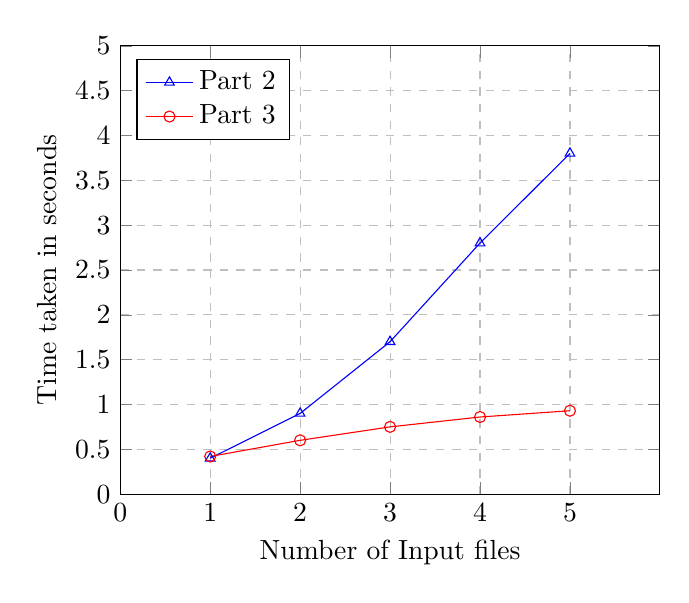
\begin{tikzpicture}
\begin{axis}[
    xlabel={Number of Input files},
    ylabel={Time taken in seconds},
    xmin=0, xmax=6,
    ymin=0, ymax=5,
    xtick={0,1,2,3,4,5},
    ytick={0,0.5,1,1.5,2,2.5,3,3.5,4,4.5,5},
    xmajorgrids=true,
    ymajorgrids=true,
    grid style=dashed,
    legend pos =north west
]

\addplot[
    color=blue,
    mark=triangle,
    ]
    coordinates {
    (1,0.4)(2,0.9)(3,1.7)(4,2.8)(5,3.8)   };
\addlegendentry{Part 2}

\addplot[
    color=red,
    mark=o,
    ]
    coordinates {
    (1,0.42)(2,0.6)(3,0.75)(4,0.86)(5,0.93)   };
\addlegendentry{Part 3}
    
\end{axis}
\end{tikzpicture}


\subsection{Table for above data}


\begin{tabularx}{0.8\textwidth} { 
  | >{\centering\arraybackslash}X 
  | >{\centering\arraybackslash}X 
  | >{\centering\arraybackslash}X |}
 \hline
 \textbf{Number of Files} & \textbf{Part 2(s)} & \textbf{Part 3(s)}  \\
 \hline
 1  & 0.4 & 0.42  \\
 2  & 0.9 & 0.6 \\
 3  & 1.7 & 0.75 \\
 4  & 2.8  & 0.86 \\
 5  & 3.8 & 0.93 \\
 
\hline
\end{tabularx}

\section{Size of files(in MB) vs time(s)}
\subsection{Graph}

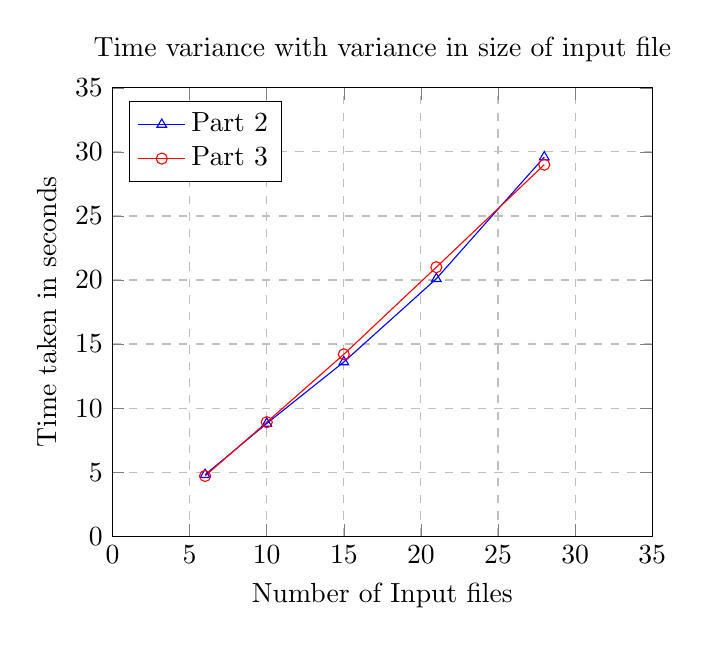
\begin{tikzpicture}
\begin{axis}[
    title={Time variance with variance in size of input file},
    xlabel={Number of Input files},
    ylabel={Time taken in seconds},
    xmin=0, xmax=35,
    ymin=0, ymax=35,
    xtick={0,5,10,15,20,25,30,35},
    ytick={0,5,10,15,20,25,30,35},
    xmajorgrids=true,
    ymajorgrids=true,
    grid style=dashed,
    legend pos =north west
]

\addplot[
    color=blue,
    mark=triangle,
    ]
    coordinates {
    (6,4.8)(10,8.8)(15,13.6)(21,20.1)(28,29.6)   };
\addlegendentry{Part 2}

\addplot[
    color=red,
    mark=o,
    ]
    coordinates {
    (6,4.7)(10,8.9)(15,14.2)(21,21)(28,29)   };
\addlegendentry{Part 3}
    
\end{axis}
\end{tikzpicture}

\subsection{Table}

\begin{tabularx}{0.8\textwidth} { 
  | >{\centering\arraybackslash}X 
  | >{\centering\arraybackslash}X 
  | >{\centering\arraybackslash}X |}
 \hline
 \textbf{Size of Files} & \textbf{Part 2(s)} & \textbf{Part 3(s)}  \\
 \hline
 6  & 4.8 & 4.7  \\
 10  & 8.8 & 8.9 \\
 15  & 13.6 & 14.2 \\
 21 & 20.1  & 21 \\
 28  & 29.6 & 29 \\
 
\hline
\end{tabularx}
\\ \\ \\ \\
\section{Taking one word repeated many times}
One word - 'banana' has been repeatedly written in the files, such that their sizes are 1,2,4,8,16 megabytes respectively 

\subsection{Graph}
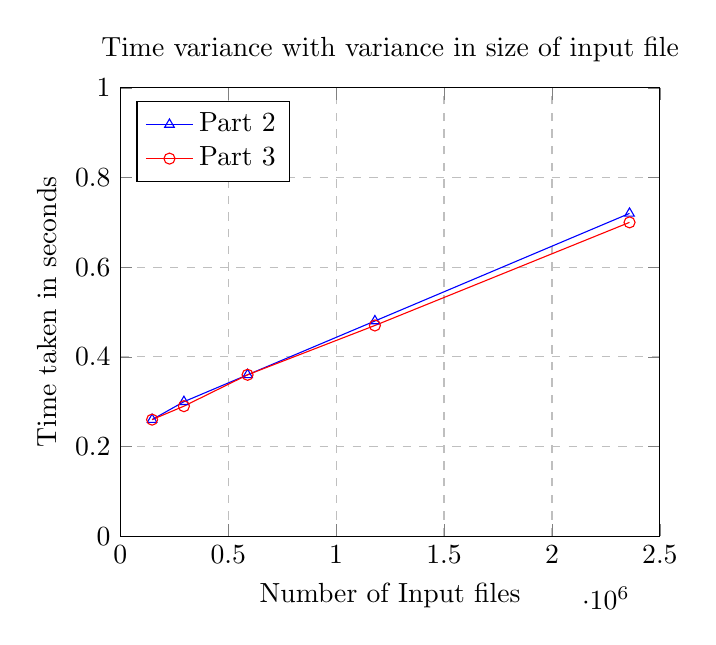
\begin{tikzpicture}
\begin{axis}[
    title={Time variance with variance in size of input file},
    xlabel={Number of Input files},
    ylabel={Time taken in seconds},
    xmin=0, xmax=2500000,
    ymin=0, ymax=1,
    xtick={0, 500000, 1000000, 1500000, 2000000,2500000},
    ytick={0,0.2,0.4,0.6,0.8,1},
    xmajorgrids=true,
    ymajorgrids=true,
    grid style=dashed,
    legend pos =north west
]

\addplot[
    color=blue,
    mark=triangle,
    ]
    coordinates {
    (147456, 0.26)(294912,0.3)(589824,0.36)(1179648,0.48)(2359296,0.72)};
\addlegendentry{Part 2}

\addplot[
    color=red,
    mark=o,
    ]
    coordinates {
    (147456, 0.26)(294912,0.29)(589824,0.36)(1179648,0.47)(2359296,0.7)};
\addlegendentry{Part 3}
    
\end{axis}
\end{tikzpicture}


\subsection{Table}

\begin{tabularx}{0.8\textwidth} { 
  | >{\centering\arraybackslash}X 
  | >{\centering\arraybackslash}X 
  | >{\centering\arraybackslash}X |}
 \hline
 \textbf{Frequency} & \textbf{Part 2(s)} & \textbf{Part 3(s)}  \\
 \hline
 147456  & 0.26 & 0.26  \\
 294912  & 0.3 & 0.29 \\
 589824  & 0.36 & 0.36 \\
 1179648  & 0.48 & 0.47 \\
 2359296  & 0.72 & 0.7 \\
 
\hline
\end{tabularx}







\section{ Tokens}
\begin{tabularx}{0.8\textwidth} { 
  | >{\centering\arraybackslash}X 
  | >{\centering\arraybackslash}X 
  | >{\centering\arraybackslash}X |}
 \hline
 \textbf{Name} & \textbf{Tokens}  \\
 \hline
 Tript  & 10 \\
 Mani  & 10 \\
 Utkarsh  & 10 \\

 
\hline
\end{tabularx}

\end{document}